\documentclass[11pt]{article}

\usepackage[a4paper,margin=1in]{geometry}
\usepackage{amsmath}
\usepackage{amssymb}
\usepackage{booktabs}
\usepackage{tabularx}
\usepackage{graphicx}
\usepackage[hidelinks]{hyperref}
\usepackage[authoryear,round]{natbib}
\usepackage{siunitx}
\usepackage{tikz}
\usetikzlibrary{arrows.meta,positioning}
\sisetup{group-separator={,}, group-minimum-digits=4}

\title{Mitigation Methods for Class Imbalance\\in Histopathology Patch Classification}
\author{Yannik Queisler}
\date{\today}

\begin{document}
\maketitle

\begin{abstract}
\noindent Class imbalance lets a patch classifier reach high aggregate accuracy while failing on rare diagnoses. This report defines six mitigation methods for histopathology patch classification and places them in the data-level, algorithm-level, and hybrid families of \citet{krawczyk2016learning}: balanced sampling and MixUp change the training data, logit adjustment and DisAlign change the objective or decision rule, and classifier re-training (cRT) and Gaussian clouded logit (GCL) adjustment combine both. All methods share one setting: a Virchow2 foundation-model encoder that is either frozen or adapted with low-rank updates, and a linear classification head. Each method is stated in its source form, with the control parameter that sets its strength and the adaptations required by this setting.
\end{abstract}

\setcounter{tocdepth}{2}
\tableofcontents
\clearpage

\section{Introduction}
\label{sec:introduction}
Diagnostic datasets in pathology are rarely balanced. Common tumour types and benign tissue dominate the training material, while the classes a diagnostic system is often meant to catch appear only a few times. A classifier trained on such data can reach high overall accuracy while its recall on rare classes stays low, because prevalence-weighted metrics reward the classes that already dominate. Long-tailed learning and medical-image evaluation literature therefore treat classwise recall, balanced accuracy, and calibration-aware probability metrics as primary outcomes under imbalance \citep{saini2023tacklingClass,zhang2023deepLong,mosquera2024classImbalance}. Mitigation methods try to raise tail-class performance without giving up the head classes, and they differ in where they intervene. This report fixes the definitions of six such methods, so that later experiments can compare them under one protocol.

\paragraph{Setting.}
All methods are defined for patch classification. Each labelled patch $x$ is embedded by the Virchow2 encoder $f_\theta$, a ViT-H/14 foundation model pretrained on pathology images \citep{zimmermann2024virchow2}, and a linear head maps the embedding to class logits $\mathbf z=W f_\theta(x)+\mathbf b$. The broader pipeline around this setting, from whole-slide imaging to patch extraction, is described in the companion datasets report \citep{queisler2026datasets}. Methods whose source form learns the representation may adapt the encoder, but only through lightweight updates. Low-rank adaptation (LoRA) keeps each pretrained weight matrix $W_0$ frozen and learns an additive update $\Delta W=BA$ of small rank $r$, applied to the attention projections \citep{hu2022lora}. Only $A$, $B$, and the head are trained, and the rest of the encoder remains fixed. This follows the evidence on adapting large pretrained models. Full fine-tuning can distort pretrained features that already generalize \citep{kumar2022fineTuning}. Under long-tailed data, heavy fine-tuning of a foundation model lowers tail-class accuracy, while lightweight fine-tuning keeps the class-conditional features consistent and performs better \citep{shi2024longTail}. The labelled patch sets are also small relative to the roughly \num{632} million encoder parameters, and small trainable adapters on frozen pathology encoders are an established way to limit overfitting in this regime \citep{hasan2025fmsWith}. Three methods train in two stages: cRT, DisAlign, and GCL. For these, stage one learns the encoder adaptation and the head, and stage two freezes the encoder together with its LoRA update and trains only the classifier or calibration parameters.

\paragraph{Notation}
Let $C$ be the number of classes and $n_c$ the number of training patches of class $c$, so that $N=\sum_{j=1}^{C}n_j$ is the training-set size and $\pi_c=n_c/N$ is the empirical prevalence of class $c$. Let $n_{\max}=\max_c n_c$. For a patch with label $y\in\{1,\ldots,C\}$, the model outputs logits $\mathbf z\in\mathbb R^{C}$ and class probabilities
\begin{equation}
  p_c=\frac{\exp(z_c)}{\sum_{j=1}^{C}\exp(z_j)}.
  \label{eq:softmax}
\end{equation}
\noindent Unless a method changes the sampler, the objective, or the decision rule, training draws patches from the empirical class distribution.

\section{Taxonomy}
\label{sec:taxonomy}
\citet{krawczyk2016learning} sorts imbalance methods into three families by what they modify. \emph{Data-level} methods change the training set or the way it is sampled, so that a standard learner sees a more balanced or more varied distribution. \emph{Algorithm-level} methods leave the data as observed and change the learner itself, through its loss, its output layer, or its decision rule, so that the learner is no longer biased toward majority classes. \emph{Hybrid} methods combine a data-level and an algorithm-level change, so that neither component alone explains their effect. Cross-entropy (CE) on the empirical distribution is the reference outside all three families: it changes neither data nor learner.

Figure~\ref{fig:taxonomy} places the six methods in these families. Two placements need a short justification. cRT and GCL are hybrid because both decouple representation learning from classifier learning, which is an algorithm-level change, and both rebalance the sampler in the classifier stage, which is a data-level change. DisAlign also trains in two stages, but its second stage keeps the sampler unchanged and rebalances only through a reweighted objective and a learned logit calibration, so it is algorithm-level.

\begin{figure}[ht]
  \centering
  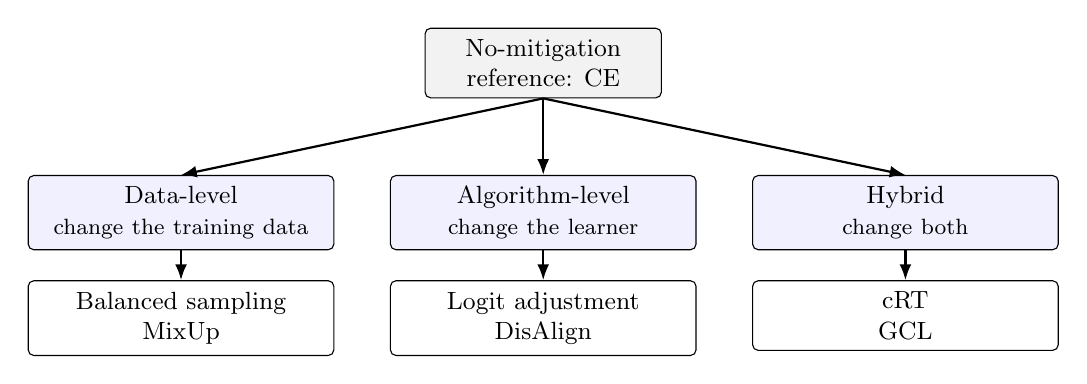
\begin{tikzpicture}[
    box/.style={draw, rounded corners=2pt, align=center, inner sep=4pt, font=\small, minimum height=0.72cm},
    baseline/.style={box, fill=gray!10, minimum width=3.0cm},
    family/.style={box, fill=blue!6, text width=3.6cm},
    method/.style={box, fill=white, text width=3.6cm},
    arrow/.style={-{Latex[length=2mm]}, thick}
  ]
    \node[baseline] (ce) at (0,0) {No-mitigation\\reference: CE};
    \node[family] (data) at (-4.6,-1.9) {Data-level\\\footnotesize change the training data};
    \node[method, below=0.38cm of data] (dataMethods) {Balanced sampling\\MixUp};
    \node[family] (alg) at (0,-1.9) {Algorithm-level\\\footnotesize change the learner};
    \node[method, below=0.38cm of alg] (algMethods) {Logit adjustment\\DisAlign};
    \node[family] (hyb) at (4.6,-1.9) {Hybrid\\\footnotesize change both};
    \node[method, below=0.38cm of hyb] (hybMethods) {cRT\\GCL};
    \draw[arrow] (ce.south) -- (data.north);
    \draw[arrow] (ce.south) -- (alg.north);
    \draw[arrow] (ce.south) -- (hyb.north);
    \draw[arrow] (data) -- (dataMethods);
    \draw[arrow] (alg) -- (algMethods);
    \draw[arrow] (hyb) -- (hybMethods);
  \end{tikzpicture}
  \caption{The six methods in the three families of \citet{krawczyk2016learning}. CE on the empirical distribution is the no-mitigation reference.}
  \label{fig:taxonomy}
\end{figure}

\section{Methods}
\label{sec:methods}
This section defines the methods in the order of Figure~\ref{fig:taxonomy}. Each definition gives the source form first and then, where needed, the thesis variant: how the method is instantiated on the Virchow2 encoder with a linear head.

\subsection{Cross-Entropy Reference}
Unweighted CE is the standard supervised objective without an imbalance correction. For a patch with label $y$, the loss is
\begin{equation}
  \mathcal L_{\mathrm{CE}}(\mathbf z,y)=-\log p_y.
  \label{eq:ce}
\end{equation}
\noindent Minibatches are drawn from the empirical distribution, so head classes contribute more loss terms per epoch than tail classes. CE is trained in the same setting as the other methods, with the same LoRA adaptation, so that each mitigation is compared with a reference that differs only in the mitigation itself.

\subsection{Data-Level Methods}
Data-level methods change what the optimizer sees and keep the CE objective. They are the simplest interventions to state, and they leave the model and its output semantics unchanged.

\subsubsection{Balanced Sampling}
Class-aware sampling fills each minibatch by first drawing a class uniformly and then drawing a patch from that class, so that every class appears at the same expected rate \citep{shen2016relayBackpropagation}. \citet{kang2020decouplingRepresentation} write this family as a power of the class count. With strength $s\in[0,1]$, patch $i$ with label $y_i$ is sampled with probability
\begin{equation}
  q_i(s)=\frac{n_{y_i}^{-s}}{\sum_{k=1}^{N}n_{y_k}^{-s}},
  \label{eq:balanced-sampling}
\end{equation}
\noindent so that class $c$ receives an expected share proportional to $n_c^{1-s}$. Setting $s=0$ recovers empirical sampling and CE; $s=1$ gives every class the same expected exposure; intermediate values rebalance partly. The loss stays Equation~\eqref{eq:ce}. Balanced sampling repeats tail patches rather than adding new ones, so at high $s$ it can overfit the few tail patches, while the head classes are seen less often per epoch.

\subsubsection{MixUp}
MixUp trains on convex combinations of random pairs of examples and their labels \citep{zhang2018mixup}. For two training patches $(x_i,y_i)$ and $(x_j,y_j)$ and a mixing weight $\lambda\sim\mathrm{Beta}(\alpha,\alpha)$, the mixed input is
\begin{equation}
  \tilde x=\lambda x_i+(1-\lambda)x_j,
  \label{eq:mixup-input}
\end{equation}
\noindent and its target is the same mixture of the two one-hot labels. With logits $\tilde{\mathbf z}$ of the mixed input, the loss is
\begin{equation}
  \mathcal L_{\mathrm{MixUp}}=\lambda\,\mathcal L_{\mathrm{CE}}(\tilde{\mathbf z},y_i)+(1-\lambda)\,\mathcal L_{\mathrm{CE}}(\tilde{\mathbf z},y_j).
  \label{eq:mixup-loss}
\end{equation}
\noindent The pair partner $j$ is a random permutation of the minibatch. The parameter $\alpha>0$ sets how strongly the pairs are mixed: as $\alpha\to0$, $\lambda$ concentrates at $0$ or $1$ and the objective returns to CE, while $\alpha=1$ draws $\lambda$ uniformly. MixUp encourages the model to behave linearly between training examples, which smooths decision boundaries and reduces overconfident predictions.

MixUp does not read class counts, and both partners are drawn from the empirical distribution. Its effect on imbalance is therefore indirect: tail patches are mixed with head patches and gain regularized neighbourhoods, but their share of the training signal is not raised. It is included as a data-level method because it enlarges the effective training set through synthetic examples, and because it is a standard baseline in long-tailed benchmarks.
\subsection{Algorithm-Level Methods}
Algorithm-level methods keep the empirical data stream and change how the learner turns features into decisions. Both methods below act on the logits: logit adjustment with a fixed shift derived from the class prior, DisAlign with a learned, input-dependent calibration.

\subsubsection{Logit Adjustment}
Logit adjustment corrects for the training prior $\pi_c$ \citep{menon2021longTail}. A classifier trained with CE estimates the training posterior, which favours head classes in proportion to their prior. Removing that prior gives decisions that suit a class-balanced target. The strength $\tau\geq0$ scales the correction, and $\tau=0$ recovers CE. In the \emph{train-time} form, the prior enters the loss:
\begin{equation}
  \mathcal L_{\mathrm{LA}}(\mathbf z,y)=-\log\frac{\exp(z_y+\tau\log\pi_y)}{\sum_{c=1}^{C}\exp(z_c+\tau\log\pi_c)}.
  \label{eq:la-train}
\end{equation}
\noindent Head classes receive a larger additive offset during training, so the model must learn a larger margin for tail classes to fit them; at inference the unadjusted logits $z_c$ are used. In the \emph{post-hoc} form, the model is trained with CE and the prior is removed only at inference:
\begin{equation}
  \hat y=\arg\max_{c}\,\bigl(z_c-\tau\log\pi_c\bigr).
  \label{eq:la-posthoc}
\end{equation}
\noindent The sign differs because the train-time form learns against prior-shifted logits, while the post-hoc form subtracts the prior from ordinary CE logits. At $\tau=1$ both target the balanced error. The post-hoc form needs no retraining and can therefore be applied to the CE model of every other method.

Either form changes the implied class prior, so the resulting probabilities are not calibrated for the natural test prevalence. Discrimination and calibration are therefore reported separately, and temperature scaling is kept distinct from prior correction.

\subsubsection{DisAlign}
Distribution alignment (DisAlign) keeps a CE-trained classifier and learns a light correction of its scores \citep{zhang2021distributionAlignment}. Stage one trains the model with CE. Stage two freezes the representation and the original head, whose logits are $z^{o}_j$, and learns for each class a scale $\alpha_j$ and a bias $\beta_j$. An input-dependent confidence $\sigma(x)=\operatorname{sigmoid}(\mathbf v^{\top}f_\theta(x))$ decides how much of the correction is applied:
\begin{equation}
  \hat z_j=\sigma(x)\bigl(\alpha_j z^{o}_j+\beta_j\bigr)+\bigl(1-\sigma(x)\bigr)z^{o}_j
         =\bigl(1+\sigma(x)\alpha_j\bigr)z^{o}_j+\sigma(x)\beta_j.
  \label{eq:disalign-calibration}
\end{equation}
\noindent Only $\alpha_j$, $\beta_j$, and $\mathbf v$ are trained, which is far fewer parameters than a new classifier. Post-hoc logit adjustment is the special case with unit scale and a fixed bias $-\tau\log\pi_j$, so DisAlign can be read as a learned, input-dependent generalization of it.

The calibration is fitted by aligning the model prediction with a reference distribution that favours balanced prediction. The reference puts weight $w_c$ on the true class of each training patch, with the generalized reweighting
\begin{equation}
  w_c(\rho)=\frac{\pi_c^{-\rho}}{\sum_{k=1}^{C}\pi_k^{-\rho}},
  \qquad
  \mathcal L_{\mathrm{DisAlign}}=-\frac{1}{N}\sum_{i=1}^{N}w_{y_i}(\rho)\log\hat p_{y_i}(x_i),
  \label{eq:disalign-loss}
\end{equation}
\noindent where $\hat p$ is the softmax of the calibrated logits $\hat{\mathbf z}$. The exponent $\rho\geq0$ is the control: $\rho=0$ weights every patch equally, $\rho=1$ gives inverse-prevalence class weights, and larger values emphasize the tail further. Stage two keeps the empirical sampler, so the rebalancing enters only through $w_c$.

\paragraph{Thesis variant.}
Stage one is the CE reference with LoRA adaptation. Stage two freezes the encoder, its LoRA update, and the linear head, and trains only the calibration parameters of Equation~\eqref{eq:disalign-calibration}. The source also reports a cosine-classifier variant; the tested variant keeps the linear head of the reference.

\subsection{Hybrid Methods}
Both hybrid methods follow the decoupling view of long-tailed learning: the representation is learned in a first stage, and a class-rebalanced sampler then corrects the classifier in a second stage in which the representation is frozen. They differ in how the first stage is trained and in how strongly the second stage rebalances.

\subsubsection{Classifier Re-Training (cRT)}
Classifier re-training separates representation learning from classifier fitting \citep{kang2020decouplingRepresentation}. Stage one trains the model with CE on the empirical distribution. Stage two freezes the learned representation $h(x)$, discards and reinitializes the linear classifier, and fits it with class-balanced sampling:
\begin{equation}
  (\widehat W,\widehat{\mathbf b})
  =\arg\min_{W,\mathbf b}\;
  \mathbb E_{(x,y)\sim q_{\mathrm{bal}}}
  \Bigl[-\log\operatorname{softmax}\bigl(W h(x)+\mathbf b\bigr)_y\Bigr],
  \label{eq:crt}
\end{equation}
\noindent where $q_{\mathrm{bal}}$ is Equation~\eqref{eq:balanced-sampling} at $s=1$. The premise is that instance-balanced training learns the best representation, and that imbalance mainly biases the classifier. cRT has no strength parameter; its rebalancing is complete by construction.

\paragraph{Thesis variant.}
The representation is $h(x)=f_\theta(x)$ with the LoRA update learned in stage one. The source also studies classifier normalization variants; the tested variant uses only the reinitialized linear classifier.

\subsubsection{Gaussian Clouded Logit (GCL) Adjustment}
GCL adjustment addresses two effects of long-tailed training in separate stages \citep{li2022gaussianClouded}. In the first stage, the embedding space is distorted: tail classes occupy a small region, and softmax saturation stops their gradients early, once the target logit is well ahead. GCL counters this by perturbing the logits with noise whose amplitude grows toward the tail. With a cosine classifier, logits are $s\cos\theta_j$, where $\theta_j$ is the angle between the feature and the class weight $\mathbf w_j$, and $s$ is a fixed scale. The clouded logit of class $j$ is
\begin{equation}
  \tilde z_j=s\bigl(\cos\theta_j-\delta_j\,\lvert\varepsilon\rvert\bigr),
  \qquad
  \delta_j=\log n_{\max}-\log n_j,
  \qquad
  \varepsilon\sim\mathcal N(0,\sigma^{2}),
  \label{eq:gcl-logit}
\end{equation}
\noindent and the model is trained with CE on $\tilde{\mathbf z}$. The most frequent class receives no noise, and tail classes receive the largest cloud size $\delta_j$. The noise always lowers the logit, so a tail patch must lie further from the class boundary before its gradient saturates; this keeps tail patches active in training and enlarges their margin. The noise scale $\sigma$ is the control: $\sigma=0$ recovers CE with a cosine classifier. At inference no noise is added.

In the second stage, the representation is frozen and the classifier is re-trained with a class-rebalanced sampler. Because GCL already lets tail patches contribute more in stage one, fully balanced sampling would over-train them. GCL instead samples class $j$ with the class-based effective number of \citet{cui2019classBalanced},
\begin{equation}
  r_j=\frac{1-\beta_j}{1-\beta_j^{\,n_j}},
  \qquad
  \beta_j=b\,\frac{\delta_j-\delta_{\min}}{\delta_{\max}-\delta_{\min}}+a,
  \label{eq:gcl-cben}
\end{equation}
\noindent normalized over classes, where $a$ and $b$ set the range $[a,a+b]$ of $\beta_j$. A larger cloud size gives a larger $\beta_j$ and hence a larger effective-number correction, so tail classes are sampled more often, but less aggressively than under uniform class sampling. The stage-two loss is again the clouded loss of Equation~\eqref{eq:gcl-logit}.

\paragraph{Thesis variant.}
Stage one trains the LoRA update and a cosine classifier head with the clouded loss. Stage two freezes the encoder and its LoRA update and re-trains only the cosine head with the sampler of Equation~\eqref{eq:gcl-cben}. The scale $s$ and the range $a,b$ are fixed before training; $\sigma$ is the tuned control. GCL replaces the linear head of the reference with a cosine head, so part of its effect may come from the head geometry rather than from the logit noise.

\section{Summary}
\label{sec:summary}
This report defines six class-imbalance mitigation methods for patch classification and places them in the three families of \citet{krawczyk2016learning}. Balanced sampling and MixUp are data-level methods, logit adjustment and DisAlign are algorithm-level methods, and cRT and GCL are hybrid methods that pair decoupled classifier learning with a rebalanced sampler. All methods except MixUp read the imbalance from the class counts $n_c$ or the prevalences $\pi_c$, and each method except cRT has one parameter that sets its strength. At zero strength, balanced sampling, MixUp, and logit adjustment reduce to CE, and GCL reduces to CE with a cosine head. The methods share one setting: a Virchow2 encoder adapted only through LoRA, a linear or cosine head, and, for the three two-stage methods, a frozen encoder in stage two. Later experiments compare them against CE with balanced accuracy, classwise recall, and probability quality, with raw and temperature-scaled outputs reported separately.

\clearpage
\bibliographystyle{plainnat}
\bibliography{references}

\end{document}
